
\section{Introduction}

Travelling Salesman Problem (TSP) is a problem with an objective to find a path that has the lowest cost. Rules are simple. Nodes that must be visited are should be visited only once and there should be no missing nodes. However this optimization problem is known as `NP-complete.' In other words, TSP has a huge search space, and it is very hard to find the optimal solution. Evolutionary method is a search algorithm based on the rules of evolution like natural selection and natural genetics\cite{golberg1989genetic}. Selection, crossover and mutation are used to improve a population of candidate solutions, and they are repeated until the terminating condition is satisfied. TSP is applicable to various fields of industry, and there have been many attempts to solve TSP \cite{fogel1993applying,banzhaf1990molecular,pereira2002gvr}. In this paper, we propose an improved crossover operator for better performance of evolutionary approach to TSP.

\section{Evolutionary Apporach to TSP}

Evolutionary approach is a heuristic search algorithm that mimics principle of evolution. Evolution of candidate solution is derived by evolutionary rules such as slection and crossover. Reproduction of offsprings mimics Darwinian {\it survival-of-the-fitness}. Therefore, individuals that have relatively low fitness values cannot participate in reproduction process. The fitness value in TSP is simple. The multiplicative inverse of the total cost of tour path can be used as the fitness value: The smaller the tour cost of a gene is, the better the gene is.

\subsection{Genetic Representation}

In order to implement a evolution-based TSP solver, solutions should be expressed as a feasible chromosome. A sequence representing the order of `city visit' is a possible solution. Suppose, for example, there are four city nodes {1,2,3,4}. The tour path 1$\rightarrow$2$\rightarrow$3$\rightarrow$4$\rightarrow$1 can then be represented with a chromosome expression $<$1,2,3,4$>$. When using evolutionary method to solve TSP, the phenotype is, in most cases, used as a chromosome for crossover. Since TSP constraints the form of valid solution, the convetional crossover with genotype expression cannot be easily implemented, and it is more difficult to devise a genotype-based crossover which rapidly converges to a sufficiently good solutions. Therefore, we also used path sequence directly as a chromosome.

\subsection{Problems in Conventional Crossover}

The solutions must contain all nodes to be visited only once and there must be no missing nodes. In conventional crossover methods, an offspring is generated by associating the some parts of chromosomes of parents. However, as shown in Fig.\ref{fig:constraintsViolation}, the conventional crossover may easily produce duplicate nodes and missing nodes.


\begin{figure}
\centering
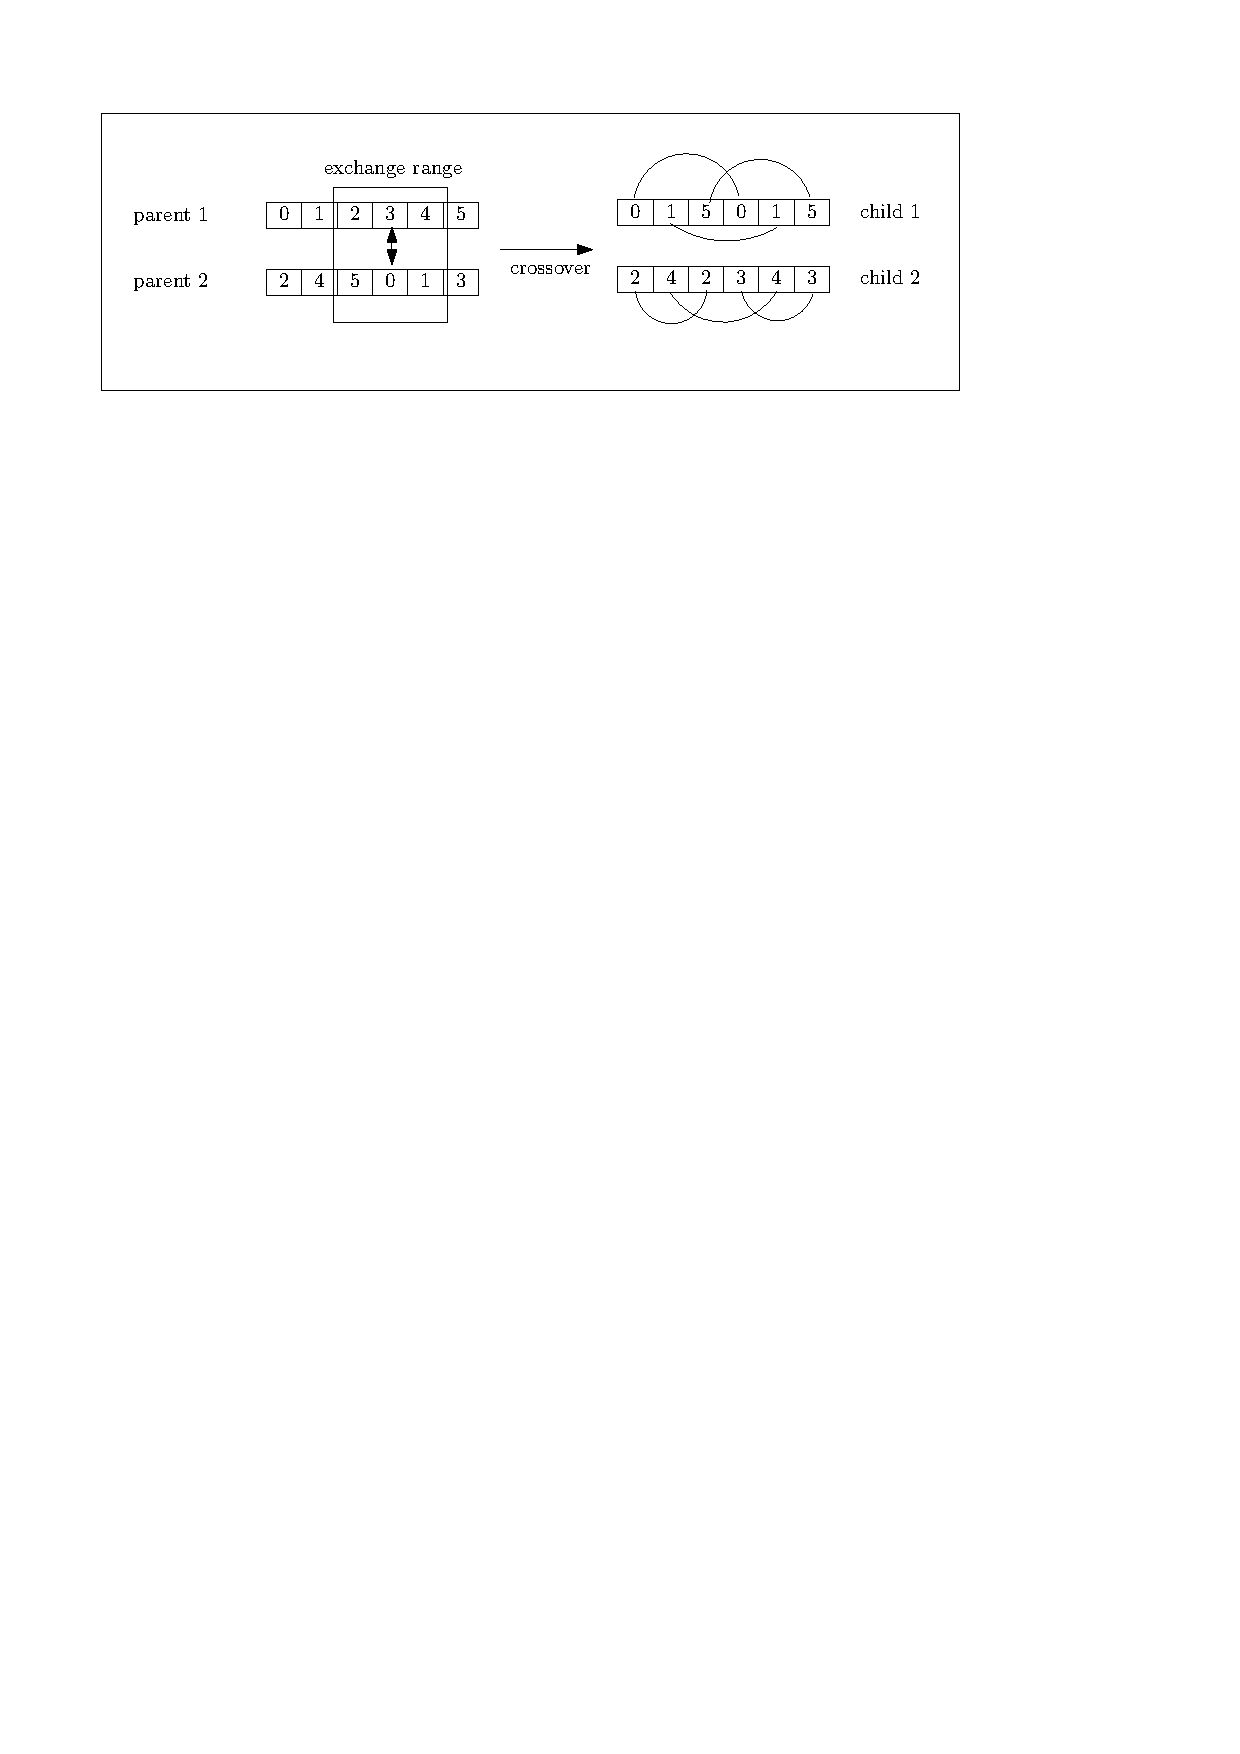
\includegraphics[width=8.0cm]{constraintsViolation.pdf}
\caption{Example of Constraints Violation by Conventional Crossover}
\label{fig:constraintsViolation}
\end{figure}

In order not to violate the constraints, many kinds of crossover operators such as `edge recombination crossover (ERX)', `generalized $n$-point crossover (GNX)' and `sequential constructive crossover (SCX)' have been proposed. Among them, so far, SCX shows the fastest convergence speed \cite{ahmed2010genetic}.

\subsection{Sequential Constructive Crossover(SCX)}

The SCX crossover method guarantees validity of offspring chromosome and conserve the merits of parents. This method tries to reduce the local distance between the adjacent nodes in the offspring chromosomes by sequentially scan the chromosomes of parents. The algorithm can be described as follows\cite{ahmed2010genetic}:

\begin{enumerate}
\item{Set the starting node 0 to be the current city $p$.}
\item{Find the two unvisited node $a$ and $b$ respectively from the chromosome of each parent by sequentially search the first unvisited node (legitimate node) after the current city $p$. If the search failed, select any unvisited node from the city template permutation such as $<$1, 2, ..., n$>$.} 
\item{Compare the distances from $p$ to $a$ ($d_{pa}$) and to $b$ ($d_{pb}$). If $d_{pa}$ is less than $d_{pb}$, add $a$ to the offspring chromosome and set $a$ to be the current node. Otherwise, $b$ is added and set to be the current node. Then go to step 2.}
\end{enumerate}

\section{Bidirectional Circular SCX}

In order to improve the performance of SCX, we propose bidirectional circular SCX (BCSCX) which can search the next possible `legitimate' nodes in the chromosomes of parents in two directions and the chromosome is regarded a circular data with no ends.

\subsection{bidirectional Property}

The BCSCX operator searches legitimate nodes in two directions. In other words, it chooses the two candidate nodes to be added to the chromosome of offspring both before and after the currently visited node from chromosome of each parent.
For example, assume that a uncompleted chromosome sequence $<$1,5$>$ has been inherited from two parents during the crossover operation. Then the current node is city 5. If, within the chromosome sequence of one parent, the city 3 is the closest unvisited node (`closest' in the aspect of the location in the sequence string) among the nodes after the current node (the city 5), and city 2 is the closest unvisited node before the current node in the sequence of one parent. The proposed BCSCX takes both nodes (cityies 3 and 2) as `legitimate candidate nodes.' Two more candidates are taken from the other parent in the similar way. Let us assume that the candidates from the other parent are city 2 and city 6. The candidates for the next node in the offspring's chromosome right after the city 5 are the union of the candidate sets (i.e., cities 2, 3, and 6), and they are tested similarly as SCX. If the cities are connected as described in Table \ref{tab:costMatrix}, $d_{56}$ is less than $d_{52}$ and $d_{53}$. Therefore, in this case, the chromosome of the offspring will grow to be $<$1,5,6$>$.


\begin{table}
\caption{The Cost Matrix with Distances between Cities}
\label{tab:costMatrix}
\begin{center}
\begin{tabular}{|c|c|c|c|c|c|c|c|}\hline
  & \sf 1 & \sf 2 & \sf 3 & \sf 4 & \sf 5 & \sf 6 & \sf 7\\ \hline
\sf 1& x & 43 & 21 & 54 & 12 & 25 & 24\\ \hline
\sf 2& 43 & x & 11 & 35 & 65 & 16 & 23\\ \hline
\sf 3& 21 & 11 & x & 43 & 27& 45 & 21\\ \hline
\sf 4& 54 & 35 & 43 & x & 83 & 31 & 33\\ \hline
\sf 5& 12 & 65 & 27 & 83 & x & 19 & 62\\ \hline
\sf 6& 25 & 16 & 45 & 31 & 19 & x & 43\\ \hline
\sf 7& 24 & 23 & 21 & 33 & 62 & 43 & x\\ \hline
\end{tabular}
\end{center}
\end{table}

\subsection{Circular Property}

SCX does not asume that chromosome strings are circulary concatenated. Therefore, if the last node of the chromosome string is the current node p, no candidate legitimate nodes can be obtained. In order to avoid this problem, SCX employed a pre-defined template. 
For example, assume that the chromosome of a parent is $<$1,3,7,6,2,4,5$>$ and that of the other is $<$1,5,7,2,6,3,4$>$, and currently constructed partial chromosome of the offspring is $<$1,5$>$. The original SCX then fails to find the legitimate node from the first parent, and the first unvisited node (in this case, city 2) from the template $<$1,2,3,4,5,6,7$>$ will be selected as the legitimate node. However, our method regards the chromosome a circular data, and jumps to the first character so that the city 3 will be selected as the legitimate node.


\subsection{Efficient Search for Legitimate Nodes}

The constructive crossovers such as SCX construct the chromosomes of offsprings by selecting the best node from the `legitimate' candidates, 
and the feasibility of the offspring chromosome is guaranteed by the `legitimacy' of the candidate nodes. However, the performance of the crossover largely depends on how to search the legitimate nodes.  Moreover, the method proposed in this paper searches the legitimate nodes in two directions, and the performance of this search process affects the overall performance of the system.

The overall performance of evolutionary TSP solver depends on three major factors: 1) $k$, the number of iteration needed for convergence to a reasonable solution, 2) $m$, the population of genes, and 3) $n$, the number of cities. If we denote the cost of the legitimate node search for constructing a child chromosome as $search(n)$, the performance of the system can be expressed as $O(km \cdot search(n))$. When a na{\"i}ve approach such as sequential search is applied, it is obvioul that $search(n)$ is $O(n^2)$ and the overall performance will be $O(kmn^2 )$. 
Since the genes converge to similar genes as the number of iterations increases, the backward search used in the method proposed in this paper inevitably requires $O(n^2)$ searches for the construction of one chromosome.

In order to resolve this problem, we employed forward and backward jump indices. The jump indices can be described as Fig.\ref{fig:jumpIndices}. In this figure, the visited nodes are shaded and the most recently visited node has thick border. The legitimate nodes are searched from this node, and the indices make it possible to search them in $O(1)$ time. 
If we consider the first chromosome state, the first five cities of offspring chromosome have been determined, and the last city is 6.
The candidates for the next city are city 8 and city 5. Therefore, the forward jump index is 2, and the backward one is 1.  
If the city 8 is selected as the next city, the jump indices have to be updated. The forward and backward indices of city 8, for example, become 1 and 3.

\begin{figure}
\centering
\includegraphics[width=5.5cm]{jumpIndices.pdf}
\caption{Example of Jump Indices and Their Modification}
\label{fig:jumpIndices}
\end{figure}

Because the solution route of TSP must return to the starting node, we assumed all the feasible chromosome starts from city 1. Let us denote the chromosome satisfying this constraints as $\chi$, and the $i$-th city in the chromosome as $\chi_i$. The forward and backward jump indices to find legitimate nodes from $\chi_i$ are denoted $f_i^{\chi}$ and $b_i^{\chi}$ respectively. The information in the chromosome of each parent before the construction of child choromosome can be initialized as shown in Table \ref{tab:initChoromosome}.

\begin{table}
\caption{The Initial Setting of Parent Chromosome before Constructive Crossorver}
\label{tab:initChoromosome}
\begin{center}
\begin{tabular}{|c|c|c|c|c|c|c|c|}\hline
$i$  & 0 & 1 & 2 & 3 & 4 & $\cdots$ & $n-1$\\ \hline
$\chi_i$ & 1 &  \multicolumn{6}{|c|}{arbitrary city permutation with (2,3,..., n) }\\ \hline
$f_i^{\chi}$  & 1 & 1 & 1 & 1 & 1 & $\cdots$ & 2\\ \hline
$b_i^{\chi}$  & 1 & 2 & 1 & 1 & 1 & $\cdots$ & 1\\ \hline
visited & Yes & No & No & No & No & $\cdots$ & No\\ \hline
\end{tabular}
\end{center}
\end{table}

Based on the circular property of the TSP solution, the indices restarts from 0 when it becomes larger than $n-1$ (i.e., $i$ mod $n$). Similarly, the indices comes down from $n-1$ when it becomes less than 0. Let us denote index $i$ satisfaying this constraints as  $<i>_n$. The node 0 (i.e., $\chi_0$) is alway 1. The forward and backward indices of all nodes are initialized as 1 except for the forward one of node $n-1$, and backward one of node $1$ because $\chi_0$ will be automatically inherited to child's choromosome and regarded an already visited node. Because BCSCX takes four candidate legitimate nodes from two parent choromosome, there is no guarantee that $\chi_1$ or $\chi_{n-1}$ will be selected as the next node. If a node $\chi_i$ is selected as the next visiting city, only two indices $f_{< i-b_i^\chi >_n}^\chi$ and $b_{< i+f_i^\chi >_n}^\chi$ in the chromosome must be updated. The update can be done as follows:

\begin{eqnarray}
\label{eq:indiceManagement}
f_{< i-b_i^\chi >_n}^\chi = & f_{< i-b_i^\chi >_n}^\chi + f_i^\chi  \\ \nonumber
b_{< i+f_i^\chi >_n}^\chi = & b_{< i+f_i^\chi >_n}^\chi  + b_i^\chi
\end{eqnarray}

With the assistance of the indices managed as shown in Eq. \ref{eq:indiceManagement}, the total search for legitimate nodes during the whole construction of child chromosome can be done in $O(n)$. Therefore, the overall system performance is $O(kmn)$, and we have only to improve the convergence speed to reduce $k$ when devising a better constructive crossover method.

\section{Experiment and Analysis}

In order to verify the validity and the efficiency of the proposed BCSCX method, we empirically compared the method with original SCX method
which is known to be superior to any other crossover methods previously proposed.
In order for the empirical comparison, we devised 4 methods and named them as follows:

\begin{itemize}
\item{{\bf SCX}: The original SCX method proposed by Ahmed\cite{ahmed2010genetic}. Two identical offsprings are created, and one of them is immediately mutated.}
\item{{\bf TWSCX}: Two-way SCX that produces two different offsprings. The first offspring $\chi^{c_1}$ is created with SCX of two parents $\chi^a$ and $\chi_b$, and another one $\chi^{c_2}$ is the crossover of $\chi^a$ and $\bar{\chi}^{b}$, the inverted string of $\chi^b$ (i.e., $\bar{\chi}^{b}_i = \chi^{b}_{n-1-i}$ ).}
\item{{\bf BCSCX}: Bidirectional circular SCX we propose.}
\item{{\bf mBCSCX}: Multi-population BCSCX. The population is subdivided into multiple gene pools, and BCSCX method is independently applied to each pool. }
\end{itemize}

As we mentioned, the bidirectional search for legitimate nodes can be a performance bottleneck if na{\"i}ve sequential search is applied.
The jump indices we introduce can significantly reduce the search time and can be also applied to any SCX-based crossover. The experiment was performed on Mac Pro machine running OS X with 2.8GHz Intel Xeon CPU and 6GB 1066MHz DDR3 ECC RAM.
Table \ref{tab:constructionTime} shows the time consumed for the construction of one child chromosome. As shown in the table our jump indices make it possible for BCSCX to work as efficiently as simple SCX. In other words, the convegence speed is more important when comparing the constructive crossover methods.


\begin{table}
\caption{Time Consumed for Single Child Chromosome Construction (in $mSec$)}
\label{tab:constructionTime}
\begin{center}
\begin{tabular}{|c|c|c|c|c|}\hline
Generation  & SCX & TWSCX & BCSCX & mBCSCX \\ \hline
1 & 1.659 & 1.924 & 2.658 & 2.673\\ \hline
2 & 1.630 & 1.928 & 2.628 & 2.597\\ \hline
3 & 1.569 & 1.858 & 2.565 & 2.555\\ \hline
4 & 1.535 & 1.888 & 2.603 & 2.579\\ \hline
\multicolumn{5}{|c|} . ... \\ \hline
40 & 1.423 & 1.600 & 2.481 & 2.492\\ \hline
\end{tabular}
\end{center}
\end{table}

\begin{figure*}
\centering
\begin{tabular}{cccc}
\includegraphics[width=4.3cm]{images/SCX4000_4Gen.jpg} &
\includegraphics[width=4.3cm]{images/TWSCX4000_4Gen.jpg} & 
\includegraphics[width=4.3cm]{images/BCSCX4000_4Gen.jpg} &
\includegraphics[width=4.3cm]{images/mBCSCX4000_4Gen.jpg} \\
(a) SCX ($d=120.89$) & (b) TWSCX $(d=76.54$) & (c) BCSCX ($d=43.92$) & (d) mBCSCX ($d=46.0$)
\end{tabular}
\caption{Convergence Comparison with 4000 cities and 4 Generations of  200 Genes}
\label{fig:ConvergenceWith4000Cities}
\end{figure*}

\begin{figure*}
\centering
\begin{tabular}{cccc}
\includegraphics[width=4.3cm]{images/conv1024_20.jpg} &
\includegraphics[width=4.3cm]{images/conv1024_100.jpg} & 
\includegraphics[width=4.3cm]{images/conv1024_400.jpg} &
\includegraphics[width=4.3cm]{images/conv1024_1000.jpg} \\
(a) 20 Genes  & (b) 100 Genes & (c) 400 Genes & (d) 1000 Genes
\end{tabular}
\caption{Convergence Comparison with Different Number of Genes for 1024 Cities}
\label{fig:ConvergenceWithDifferentGenes}
\end{figure*}


For the experiment, we generated randomly located $n$ cities on 2D plane and the cost from a city to another was computed as Euclidean distance on the plane. Fig. \ref{fig:ConvergenceWith4000Cities} compares the convergence speed of the four methods in the early stage of the evolution (only four generations). In this experiment, 4000 cities are given and 200 genes are evolved. After only four generations, BCSCX and mBCSCX produced very reasonable solution. In other words, the bidirectional search for legitimate nodes helps the gene population converge efficiently to acceptable solutions. After four generations, the lengths (the sum of distances between adjacent cities) of the routes are 120.89, 76.54, 43.92 and 46.0 for SCX, TWSCX, BCSCX and mBCSCX respectively. The BCSCX method showed the best convergence speed as shown in the figure. 


Fig.\ref{fig:ConvergenceWithDifferentGenes} shows the convergence speed with various size of population. Each experiment used 1024 random cities, and the number of genes was 20, 100, 400 and 1000 for (a), (b), (c) and (d) respectively. In any case, BCSCX showed the most rapid convergence. More importantly, the fast convergence of BCSCX does not largely depend on the size of population. In other words, it would be better to divide population into smaller groups to maintain the variety of genes and utilize the parallel computing power of current computer architecture. Therefore, mBCSCX will be very useful for long-term evolution for larger problems.

The convergence trends of the long-term evolution are also visualized as shown in Fig. \ref{fig:longTermEvolution}. In this experiment, 50 genes are evolved to find the route for 100 cities. BCSCX converges fast but immediately stays at a local minimum. However, mBCSCX shows slightly slower convergence than BCSCX, but it continues to improve the result during the whole evolution period. Although the original SCX also continuously improves the result, its convergence speed is too slow compared to BCSCX or mBCSCX. TWSCX stays at a worse local minimum compared to BCSCX and mBCSCX.



\section{Conclusion}


In this paper, we proposed an improved crossover operator (BCSCX) based on the sequential constructive crossover (SCX). Since TSP constrains the offspring chromosome, many special crossover methods that do not violate the constraints have been proposed. Among those methods, it is known that SCX shows the best performance.
However, SCX does not exploit the symmetry of the problem. When we handle symmetric TSPs, the search directions for legitimate nodes may be forward and backward, and the solution paths obtained from TSP are naturally circular. We extended SCX to take those aspects into account, and the proposed BCSCX showed better performance.
Moreover, the accuracy and the efficiency of BCSCX-based evolution were not greatly influenced by the population size. Therefore, interestingly, multi- population version of BCSCX (mBCSCX) showed slightly slower convergence speed while it yielded better solutions than single-population BCSCX.
Those results mean population size plays a less important role than expected. In other words, the better performance will be obtained when the diversity of the genes in the population is maintained and the evolution is not trapped in a local minimum. This implies that BCSCX can be successfully applied to parallel processing frameworks to find better solution in shorter time in an mBCSCX-like way.

\begin{figure}
\centering
\label{fig:longTermEvolution}
\includegraphics[width=9.0cm]{images/longtermEvolve.jpg} 
\caption{Long-term Convergence Graph (1,000 Generations with 50 Genes for 100 cities) of Different Crossover Methods}
\end{figure}


\section*{Acknowlegment}

Acknowledgment is hidden in the manuscript for review.
%This work was supported in part by ETRI R\&D Program (“Development of Big Data Platform for Dual Mode Batch-Query Analytics, 14ZS1400”) and %also in part by Brain Busan 21 (BB21) support program supervised by Busan Human Resources Development Institute.